\chapter{Preliminaries}\label{chap:preliminaries}

\section{General Notation}

We'll refer to \(\reals\) for the reals, \(\utri\) represents
the unit triangle (or unit simplex) in \(\reals^2\):
\(\utri = \left\{(s, t) \mid 0 \leq s, t, s + t \leq 1\right\}\).
When dealing with sequences with multiple indices, e.g.
\(s_{m, n} = m + n\), we'll use bold symbols to represent
a multi-index: \(\bm{i} = (m, n)\). We'll use \(\left|\bm{i}\right|\) to
represent the sum of the components in a multi-index.
The binomial coefficient
\(\binom{n}{k}\) is equal to \(\frac{n!}{k! (n - k)!}\) and the trinomial
coefficient \(\binom{n}{i, j, k}\) is equal to \(\frac{n!}{i! j! k!}\)
(where \(i + j + k = n\)). The notation \(\delta_{ij}\) represents the
Kronecker delta, a value which is \(1\) when \(i = j\) and \(0\)
otherwise.

\section{Floating Point and Forward Error Analysis}

We assume all floating point operations obey
\begin{equation}
  a \star b = \fl{a \circ b} = (a \circ b)(1 + \delta_1) =
  (a \circ b) / (1 + \delta_2)
\end{equation}
where \(\star \in \left\{\oplus, \ominus, \otimes, \oslash\right\}\), \(\circ
\in \left\{+, -, \times, \div\right\}\) and \(\left|\delta_1\right|,
\left|\delta_2\right| \leq \mach\). The symbol \(\mach\) is the unit round-off
and \(\star\) is a floating point operation, e.g.
\(a \oplus b = \fl{a + b}\). (For IEEE-754 floating point double precision,
\(\mach = 2^{-53}\).) We denote the computed result of
\(\alpha \in \reals\) in floating point arithmetic by
\(\widehat{\alpha}\) or \(\fl{\alpha}\) and use \(\floats\) as the set of
all floating point numbers (see \cite{Higham2002} for more details).
Following \cite{Higham2002}, we will use the following classic properties in
error analysis.

\begin{enumerate}
  \item If \(\delta_i \leq \mach\), \(\rho_i = \pm 1\), then
      \(\prod_{i = 1}^n (1 + \delta_i)^{\rho_i} = 1 + \theta_n\),
  \item \(\left|\theta_n\right| \leq \gamma_n \coloneqq
      n \mach / (1 - n \mach)\),
  \item \((1 + \theta_k)(1 + \theta_j) = 1 + \theta_{k + j}\),
  \item \(\gamma_k + \gamma_j + \gamma_k \gamma_j \leq \gamma_{k + j}
    \Longleftrightarrow (1 + \gamma_k)(1 + \gamma_j) \leq 1 + \gamma_{k + j}\),
  \item \((1 + \mach)^j \leq 1 / (1 - j \mach) \Longleftrightarrow
  (1 + \mach)^j - 1 \leq \gamma_j\).
\end{enumerate}

\section{B\'{e}zier Curves}

A \textbf{B\'{e}zier curve} is a mapping from the unit interval
that is determined by a set of control points
\(\left\{\bm{p}_j\right\}_{j = 0}^n \subset \reals^d\).
For a parameter \(s \in \left[0, 1\right]\), there is a corresponding
point on the curve:
\begin{equation}
b(s) = \sum_{j = 0}^n \binom{n}{j} (1 - s)^{n - j} s^j \bm{p}_j \in
  \reals^d.
\end{equation}
This is a combination of the control points weighted by
each Bernstein basis function
\(B_{j, n}(s) = \binom{n}{j} (1 - s)^{n - j} s^j\).
Due to the binomial expansion
\(1 = (s + (1 - s))^n = \sum_{j = 0}^n B_{j, n}(s)\),
a Bernstein basis function is in
\(\left[0, 1\right]\) when \(s\) is as well. Due to this fact, the
curve must be contained in the convex hull of it's control points.

\subsection{de Casteljau Algorithm}

Next, we recall\footnote{We have used slightly non-standard notation for the
terms produced by the de Casteljau algorithm: we start the superscript at
\(n\) and count down to \(0\) as is typically done when describing Horner's
algorithm. For example, we use \(b_j^{(n - 2)}\) instead of
\(b_j^{(2)}\).} the de Casteljau algorithm:

\begin{breakablealgorithm}
  \caption{\textit{de Casteljau algorithm for polynomial evaluation.}}
  \label{alg:de-casteljau}

  \begin{algorithmic}
    \Function{\(\mathtt{result} = \mathtt{DeCasteljau}\)}{$b, s$}
      \State \(n = \texttt{length}(b) - 1\)
      \State \(\widehat{r} = 1 \ominus s\)
      \\
      \For{\(j = 0, \ldots, n\)}
        \State \(\widehat{b}_j^{(n)} = b_j\)
      \EndFor
      \\
      \For{\(k = n - 1, \ldots, 0\)}
        \For{\(j = 0, \ldots, k\)}
          \State \(\widehat{b}_j^{(k)} = \left(
              \widehat{r} \otimes \widehat{b}_j^{(k + 1)}\right) \oplus
              \left(s \otimes \widehat{b}_{j + 1}^{(k + 1)}\right)\)
        \EndFor
      \EndFor
      \\
      \State \(\mathtt{result} = \widehat{b}_0^{(0)}\)
    \EndFunction
  \end{algorithmic}
\end{breakablealgorithm}

\begin{theorem}[\cite{Mainar1999}, Corollary 3.2]
If \(p(s) = \sum_{j = 0}^n b_j B_{j, n}(s)\) and \(\mathtt{DeCasteljau}(p, s)\)
is the value computed by the de Casteljau algorithm then\footnote{In the
original paper the factor on \(\widetilde{p}(s)\) is \(\gamma_{2n}\),
but the authors did not consider round-off when computing
\(1 \ominus s\).}
\begin{equation}
\left|p(s) - \mathtt{DeCasteljau}(p, s)\right| \leq \gamma_{3n}
\sum_{j = 0}^n \left|b_j\right| B_{j, n}(s).
\end{equation}
\end{theorem}

The relative condition number of the evaluation of \(p(s) = \sum_{j = 0}^n
b_j B_{j, n}(s)\) in Bernstein form used in this work is (see
\cite{Mainar1999, Farouki1987}):
\begin{equation}
\cond{p, s} = \frac{\widetilde{p}(s)}{\left|p(s)\right|},
\end{equation}
where
\(\widetilde{p}(s) \coloneqq \sum_{j = 0}^n \left|b_j\right| B_{j, n}(s)\).

To be able to express the algorithm in matrix form, we define
the vectors
\begin{equation}
b^{(k)} = \left[\begin{array}{c c c} b_0^{(k)} & \cdots &
b_k^{(k)}\end{array}\right]^T, \quad
\widehat{b}^{(k)} = \left[\begin{array}{c c c} \widehat{b}_0^{(k)} & \cdots &
    \widehat{b}_k^{(k)}\end{array}\right]^T
\end{equation}
and the reduction matrices:
\begin{equation}
U_k = U_k(s) = \left[\begin{array}{c c c c c c}
    1 - s  & s      & 0      & \cdots & \cdots & 0      \\
    0      & 1 - s  & s      & \ddots &        & \vdots \\
    \vdots & \ddots & \ddots & \ddots & \ddots & \vdots \\
    \vdots &        & \ddots & \ddots & \ddots & 0 \\
    0      & \cdots & \cdots & 0      & 1 - s  & s
\end{array}\right] \in \reals^{k \times (k + 1)}.
\end{equation}
With this, we can express (\cite{Mainar1999}) the de Casteljau algorithm as
\begin{equation}\label{eq:matrix-de-casteljau}
b^{(k)} = U_{k + 1} b^{(k + 1)}
\Longrightarrow b^{(0)} = U_1 \cdots U_n b^{(n)}.
\end{equation}

In general, for a sequence \(v_0, \ldots, v_n\) we'll refer to \(v\)
as the vector containing all of the values:
\(v = \left[\begin{array}{c c c} v_0 & \cdots &
    v_n\end{array}\right]^T.\)

\section{B\'{e}zier Triangles}

A \textbf{B\'{e}zier triangle} (\cite[Chapter~17]{Farin2001}) is a
mapping from the unit triangle
\(\utri\) and is determined by a control net
\(\left\{\bm{p}_{i, j, k}\right\}_{i + j + k = n} \subset \reals^d\).
A B\'{e}zier triangle is a particular kind of B\'{e}zier surface, i.e. one
in which there are two cartesian or three barycentric input parameters.
Often the term B\'{e}zier surface is used to refer to a tensor product or
rectangular patch.
For \((s, t) \in \utri\) we can define barycentric weights
\(\lambda_1 = 1 - s - t, \lambda_2 = s, \lambda_3 = t\) so that
\begin{equation}
1 = \left(\lambda_1 + \lambda_2 + \lambda_3\right)^n =
  \sum_{\substack{i + j + k = n \\ i, j, k \geq 0}} \binom{n}{i, j, k}
  \lambda_1^i \lambda_2^j \lambda_3^k.
\end{equation}
Using this we can similarly define a (triangular) Bernstein basis
\begin{equation}
B_{i, j, k}(s, t) = \binom{n}{i, j, k} (1 - s - t)^i s^j t^k
  = \binom{n}{i, j, k} \lambda_1^i \lambda_2^j \lambda_3^k
\end{equation}
that is in \(\left[0, 1\right]\) when \((s, t)\) is in \(\utri\).
Using this, we define points on the B\'{e}zier triangle as a
convex combination of the control net:
\begin{equation}
b(s, t) = \sum_{i + j + k = n} \binom{n}{i, j, k}
  \lambda_1^i \lambda_2^j \lambda_3^k
  \bm{p}_{i, j, k} \in \reals^d.
\end{equation}

\begin{figure}
  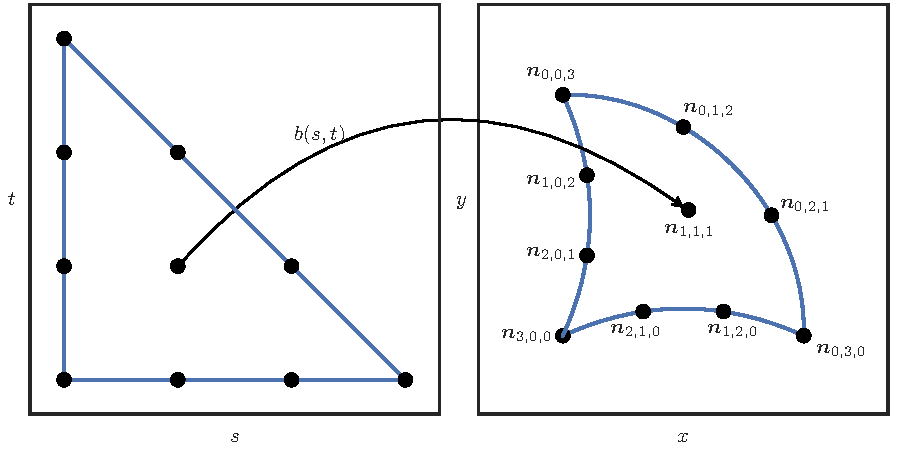
\includegraphics{../images/data-transfer/main_figure01.pdf}
  \centering
  \captionsetup{width=.75\linewidth}
  \caption{Cubic B\'{e}zier triangle}
  \label{fig:cubic-bezier-example}
\end{figure}

\noindent Rather than defining a B\'{e}zier triangle by the control net, it can
also be uniquely determined by the image of a standard lattice of
points in \(\utri\): \(b\left(j/n, k/n\right) = \bm{n}_{i, j, k}\);
we'll refer to these as \textbf{standard nodes}.
Figure~\ref{fig:cubic-bezier-example} shows these standard nodes for
a cubic triangle in \(\reals^2\). To see the correspondence,
when \(p = 1\) the standard nodes \textbf{are} the control net
\begin{equation}
b(s, t) = \lambda_1 \bm{n}_{1, 0, 0} +
\lambda_2 \bm{n}_{0, 1, 0} + \lambda_3 \bm{n}_{0, 0, 1}
\end{equation}
and when \(p = 2\)
\begin{multline}
b(s, t) = \lambda_1\left(2 \lambda_1 - 1\right) \bm{n}_{2, 0, 0} +
\lambda_2\left(2 \lambda_2 - 1\right) \bm{n}_{0, 2, 0} +
\lambda_3\left(2 \lambda_3 - 1\right) \bm{n}_{0, 0, 2} + \\
4 \lambda_1 \lambda_2 \bm{n}_{1, 1, 0} +
4 \lambda_2 \lambda_3 \bm{n}_{0, 1, 1} +
4 \lambda_3 \lambda_1 \bm{n}_{1, 0, 1}.
\end{multline}
However, it's worth noting that the transformation between
the control net and the standard nodes has condition
number that grows exponentially with \(n\) (see \cite{Farouki1991}, which
is related but does not directly show this).
This may make working with
higher degree triangles prohibitively unstable.

A \textbf{valid} B\'{e}zier triangle is one which is
diffeomorphic to \(\utri\), i.e. \(b(s, t)\) is bijective and has
an everywhere invertible Jacobian. We must also have the orientation
preserved, i.e. the Jacobian must have positive determinant. For example, in
Figure~\ref{fig:inverted-element}, the image of \(\utri\) under
the map \(b(s, t) = \left[\begin{array}{c c} (1 - s - t)^2 + s^2 & s^2 + t^2
\end{array}\right]^T\) is not valid because the Jacobian is zero along
the curve \(s^2 - st - t^2 - s + t = 0\) (the dashed line). Elements that
are not valid are called \textbf{inverted} because they have regions with
``negative area''. For the example, the image \(b\left(\utri\right)\)
leaves the boundary determined by the edge curves: \(b(r, 0)\),
\(b(1 - r, r)\) and \(b(0, 1 - r)\) when \(r \in \left[0, 1\right]\).
This region outside the boundary is traced twice, once with
a positive Jacobian and once with a negative Jacobian.
\begin{figure}
  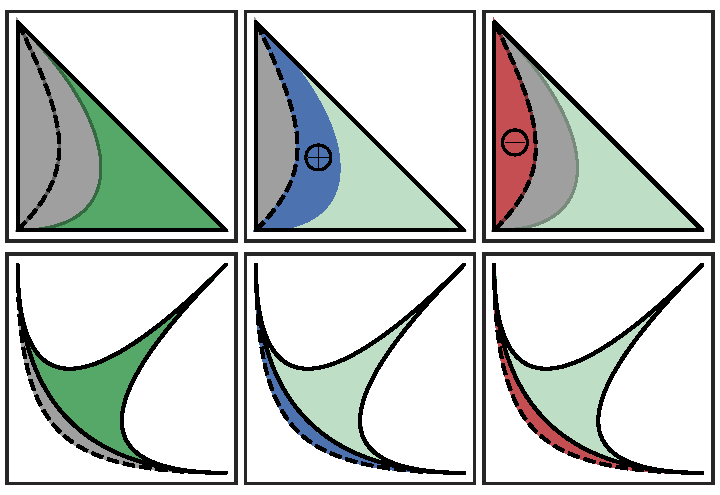
\includegraphics{../images/data-transfer/inverted_element.pdf}
  \centering
  \captionsetup{width=.75\linewidth}
  \caption{The B\'{e}zier triangle given by \(b(s, t) = \left[
    (1 - s - t)^2 + s^2 \; \; s^2 + t^2 \right]^T\) produces an
    inverted element. It traces the same region twice, once with
    a positive Jacobian (the middle column) and once with a negative
    Jacobian (the right column).}
  \label{fig:inverted-element}
\end{figure}

\section{Curved Elements}\label{sec:curved-elements}

We define a curved mesh element \(\mathcal{T}\) of degree \(p\)
to be a B\'{e}zier triangle in \(\reals^2\) of the same degree.
We refer to the component functions of \(b(s, t)\) (the map that
gives \(\mathcal{T} = b\left(\utri\right)\)) as \(x(s, t)\) and \(y(s, t)\).

This fits a typical definition (\cite[Chapter~12]{FEM-ClaesJohnson})
of a curved element, but gives a special meaning to the mapping from
the reference triangle. Interpreting elements as B\'{e}zier triangles
has been used for Lagrangian methods where
mesh adaptivity is needed (e.g. \cite{CardozeMOP04}). Typically curved
elements only have one curved side (\cite{McLeod1972}) since they are used
to resolve geometric features of a boundary. See also
\cite{Zlmal1973, Zlmal1974}.
B\'{e}zier curves and triangles have a number of mathematical properties
(e.g. the convex hull property) that lead to elegant geometric
descriptions and algorithms.

Note that a B\'{e}zier triangle can be
determined from many different sources of data (for example the control net
or the standard nodes). The choice of this data may be changed to suit the
underlying physical problem without changing the actual mapping. Conversely,
the data can be fixed (e.g. as the control net) to avoid costly basis
conversion; once fixed, the equations of motion and other PDE terms can
be recast relative to the new basis (for an example, see \cite{Persson2009},
where the domain varies with time but the problem is reduced to
solving a transformed conservation law in a fixed reference configuration).

\subsection{Shape Functions}\label{subsec:shape-functions}

When defining shape functions (i.e. a basis with geometric meaning) on a
curved element there are (at least) two choices. When the degree of the
shape functions is the same as the degree of the function being
represented on the B\'{e}zier triangle,
we say the element \(\mathcal{T}\) is \textbf{isoparametric}.
For the multi-index
\(\bm{i} = (i, j , k)\), we define \(\bm{u}_{\bm{i}} =
\left(j/n, k/n\right)\) and the corresponding standard node
\(\bm{n}_{\bm{i}} = b\left(\bm{u}_{\bm{i}}\right)\).
Given these points, two choices for shape functions present
themselves:
\begin{itemize}
  \itemsep 0em
  \item \textbf{Pre-Image Basis}:
    \(\phi_{\bm{j}}\left(\bm{n}_{\bm{i}}\right) =
      \widehat{\phi}_{\bm{j}}\left(\bm{u}_{\bm{i}}\right) =
      \widehat{\phi}_{\bm{j}}\left(b^{-1}\left(
      \bm{n}_{\bm{i}}\right)\right)\)
    where \(\widehat{\phi}_{\bm{j}}\) is a canonical basis function
    on \(\utri\), i.e.
    \(\widehat{\phi}_{\bm{j}}\) a degree \(p\) bivariate polynomial and
    \(\widehat{\phi}_{\bm{j}}\left(\bm{u}_{\bm{i}}\right) =
    \delta_{\bm{i} \bm{j}}\)
  \item \textbf{Global Coordinates Basis}:
    \(\phi_{\bm{j}}\left(\bm{n}_{\bm{i}}\right) =
    \delta_{\bm{i} \bm{j}}\), i.e. a canonical basis function
    on the standard nodes \(\left\{\bm{n}_{\bm{i}}\right\}\).
\end{itemize}

\noindent For example, consider a quadratic B\'{e}zier triangle:
\begin{gather}
b(s, t) = \left[ \begin{array}{c c}
    4 (s t + s + t) & 4 (s t + t + 1)
  \end{array}\right]^T \\
\Longrightarrow
\left[ \begin{array}{c c c c c c}
    \bm{n}_{2, 0, 0} &
    \bm{n}_{1, 1, 0} &
    \bm{n}_{0, 2, 0} &
    \bm{n}_{1, 0, 1} &
    \bm{n}_{0, 1, 1} &
    \bm{n}_{0, 0, 2}
  \end{array}\right] = \left[ \begin{array}{c c c c c c}
    0 & 2 & 4 & 2 & 5 & 4 \\
    4 & 4 & 4 & 6 & 7 & 8
  \end{array}\right].
\end{gather}
In the \textbf{Global Coordinates Basis}, we have
\begin{equation}
\phi^{G}_{0, 1, 1}(x, y) = \frac{(y - 4) (x - y + 4)}{6}.
\end{equation}
For the \textbf{Pre-Image Basis}, we need the inverse
and the canonical basis
\begin{equation}
b^{-1}(x, y) = \left[ \begin{array}{c c}
    \frac{x - y + 4}{4} & \frac{y - 4}{x - y + 8}
  \end{array}\right] \quad \text{and} \quad
\widehat{\phi}_{0, 1, 1}(s, t) = 4 s t
\end{equation}
and together they give
\begin{equation}
\phi^{P}_{0, 1, 1}(x, y) = \frac{(y - 4) (x - y + 4)}{x - y + 8}.
\end{equation}
In general \(\phi_{\bm{j}}^P\) may not even be a rational bivariate
function; due to composition with \(b^{-1}\) we can only guarantee that
it is algebraic (i.e. it can be defined as the zero set of polynomials).

\subsection{Curved Polygons}\label{subsec:curved-polygons}

\begin{figure}
  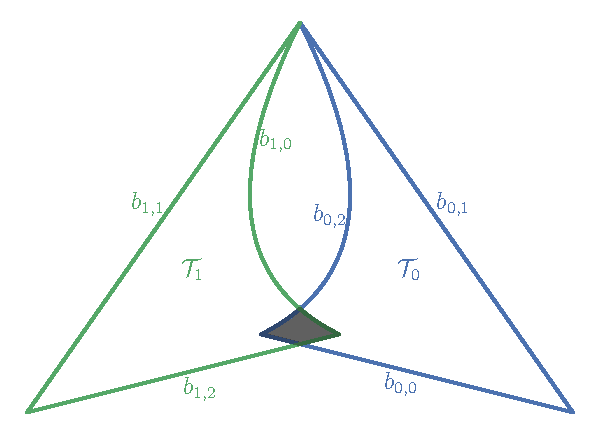
\includegraphics{../images/data-transfer/main_figure26.pdf}
  \centering
  \captionsetup{width=.75\linewidth}
  \caption{Intersection of B\'{e}zier triangles form a curved polygon.}
  \label{fig:bezier-triangle-intersect}
\end{figure}

When intersecting two curved elements, the resulting surface(s) will
be defined by the boundary, alternating between edges of each
element.
For example, in Figure~\ref{fig:bezier-triangle-intersect}, a
``curved quadrilateral'' is formed when two B\'{e}zier triangles
\(\mathcal{T}_0\) and \(\mathcal{T}_1\) are intersected.

A \textbf{curved polygon} is defined by a collection of B\'{e}zier curves
in \(\reals^2\) that determine the boundary. In order to be
a valid polygon, none of the boundary curves may cross, the
ends of consecutive edge curves must meet and the curves must be right-hand
oriented. For our example in
Figure~\ref{fig:bezier-triangle-intersect}, the triangles
have boundaries formed by three B\'{e}zier curves:
\(\partial \mathcal{T}_0 = b_{0, 0} \cup b_{0, 1} \cup b_{0, 2}\) and
\(\partial \mathcal{T}_1 = b_{1, 0} \cup b_{1, 1} \cup b_{1, 2}\).
The intersection \(\mathcal{P}\) is defined by four boundary
curves: \(\partial \mathcal{P} =
C_1 \cup C_2 \cup C_3 \cup C_4\). Each boundary
curve is itself a B\'{e}zier curve\footnote{A specialization of a
B\'{e}zier curve \(b\left(\left[a_1, a_2\right]\right)\)
is also a B\'{e}zier curve.}:
\(C_1 = b_{0, 0}\left(\left[0, 1/8\right]\right)\),
\(C_2 = b_{1, 2}\left(\left[7/8, 1\right]\right)\),
\(C_3 = b_{1, 0}\left(\left[0, 1/7\right]\right)\) and
\(C_4 = b_{0, 2}\left(\left[6/7, 1\right]\right)\).

Though an intersection can be described in terms of the B\'{e}zier triangles,
the structure of the control net will be lost. The region will not in general
be able to be described by a mapping from a simple space like
\(\utri\).

\section{Error-Free Transformation}

An error-free transformation is a computational method where both
the computed result and the round-off error are returned. It
is considered ``free'' of error if the round-off can be represented
exactly as an element or elements of \(\floats\).
The error-free transformations used in this work are
the \texttt{TwoSum} algorithm by Knuth (\cite{Knuth1997}) and
\texttt{TwoProd} algorithm by Dekker (\cite{Dekker1971}, Section 5),
respectively.

\begin{theorem}[\cite{Ogita2005}, Theorem 3.4]\label{thm:eft}
For \(a, b \in \floats\) and \(P, \pi, S, \sigma \in \floats\),
\texttt{TwoSum} and \texttt{TwoProd} satisfy
\begin{alignat}{4}
\left[S, \sigma\right] &= \mathtt{TwoSum}(a, b), & \, S &= \fl{a + b},
  S + \sigma &= a + b, \sigma &\leq \mach \left|S\right|,
  & \, \sigma &\leq \mach \left|a + b\right| \\
\left[P, \pi\right] &= \mathtt{TwoProd}(a, b),
  & \, P &= \fl{a \times b}, P + \pi &= a \times b,
  \pi &\leq \mach \left|P\right|,
  & \, \pi &\leq \mach \left|a \times b\right|.
\end{alignat}
The letters \(\sigma\) and \(\pi\) are used to indicate that the
errors came from sum and product, respectively. See
Appendix~\ref{chap:appendix-algo} for implementation details.
\end{theorem}
